\documentclass[a4paper,12pt]{report}
%\documentclass[a4paper,10pt]{scrartcl}

\usepackage[utf8]{inputenc}
\usepackage[T1]{fontenc}
\usepackage{graphicx}
\usepackage{hyperref}
\usepackage{xcolor}


\usepackage[margin=0.75in]{geometry}

\renewcommand{\contentsname}{Sommaire}

\renewcommand{\chaptername}{}
\setcounter{chapter}{-1}


\title{\Huge Rapport \\ 
	Projet de compilation avancée \\
	\large Développement d'un interpréteur pour le langage UM de la machine universelle \\
	Développement d'un compilateur du langage S-UM vers le langage UM}
\author{Amel ARKOUB 3301571 \\ Ling-Chun SO 3414546}
\date{04 avril 2018}

\pdfinfo{
  /Title    ()
  /Author   ()
  /Creator  ()
  /Producer ()
  /Subject  ()
  /Keywords ()
}

\begin{document}
\maketitle

\tableofcontents
\newpage

\chapter{Introduction}
\section{Présentation}
Le projet se divise en deux parties. Dans un premier temps, nous fournissons une implantation de la machine universelle (\url{www.boundvariable.org/um-spec.txt})
issue du concours de programmation \textit{ACM International Conference on Functional Programming} (ICFP) de 2006 
(\url{www.boundvariable.org/task.shtml}).
Nous souhaiterions également pouvoir programmer dans le langage compris par la machine universelle, ce qui n'est pas chose aisée car il s'agit là d'un langage
binaire. Ainsi dans un second temps nous allons écrire un compilateur du langage S-UM 
\textit{Specification of Universal Machine} vers le langage binaire UM.

\section{Description des fichiers}
Voici les différents dossiers et ce qu'ils contiennent :
\begin{itemize}
 \item ./um/ $\rightarrow$ Ce dossier contient l'implantation de la machine universelle.
 \item ./sum/ $\rightarrow$ Ce dossier contient l'implantation du compilateur S-UM.
 \item ./tests/ $\rightarrow$ Ce dossier contient les différents tests du compilateur S-UM.
 \item ./rapport.pdf $\rightarrow$ Ce fichier est le rapport même.
 \item ./README.md $\rightarrow$ Ce fichier contient les instructions pour compiler et tester le projet.
 \item ./rapport/ $\rightarrow$ Ce dossier contient les sources de ce rapport en LateX.
 \item ./archives/ $\rightarrow$ Ce dossier contient essentiellement des fichiers à ne pas considérer. Il s'agit d'un début d'analyseur/parseur en C pour le langage S-UM et d'une implantation de la machine universelle manipulant des listes de tableaux. En effet, pour des raisons de performances, nous avons décidé de l'abandonner pour une implantation manipulant des tableaux de tableaux.
\end{itemize}


\section{Etat du projet}
Le projet est dans l'ensemble terminé, cependant certains points sont à préciser:
\begin{itemize}
 \item la machine universelle (UM): \textcolor{green}{Fonctionnel}
 \item le compilateur S-UM: \textcolor{green}{Fonctionnel}
 \\ Tous les traits du langage sont supportés mais il est important de préciser:
 \begin{itemize}
  \item séquence d'instructions : \textcolor{green}{Fonctionnel}
  \item affectation de variable : \textcolor{green}{Fonctionnel}
  \item print : \textcolor{orange}{Améliorable}
  \\ En effet, le print fonctionne pour les chaînes de caractères et ainsi que les constantes, cependant elle n'affiche que l'évaluation
  modulo 256. Par exemple, \textit{print 96+1} affichera en sortie ``a'', 97 étant la lettre ``a'' en ASCII.
  \item scan : \textcolor{orange}{Améliorable}
  \\Le scan ne prend qu'un caractère ASCII.
  \item alternative : \textcolor{green}{Fonctionnel}
  \item entier : \textcolor{green}{Fonctionnel}
  \item chaine de caractères : \textcolor{green}{Fonctionnel}
  \item expressions arithmétiques : \textcolor{green}{Fonctionnel}
  \item expressions relationnelles : \textcolor{green}{Fonctionnel}
  \item expressions logiques binaires : \textcolor{green}{Fonctionnel}
  \item expressions logiques unaires : \textcolor{green}{Fonctionnel}
 \end{itemize}
\end{itemize}


\chapter{Machine Universelle}
\section{Structure}
Au niveau de l'implantation de la machine universelle, étant donné que chaque \textit{platter} est codé sur 32 bits, nous utilisons
un entier non signé 32 bits :
\begin{verbatim}
 typedef uint32_t uint32;
\end{verbatim}

pour contenir les instructions du programme, nous avons choisi la structure suivante :
\begin{verbatim}
typedef struct array{
  uint32 size;
  uint32 *platter;
} array;
\end{verbatim}
C'est une structure permet de contenir un tableau d'instructions et la taille mémoire du tableau (cette dernière est nécessaire lors de
l'instruction LOAD PROGRAM).
\\ \\
Afin de pouvoir garder en mémoire tous les indices réutilisables du tableau, nous avons une structure de liste pour les indices. Dans le cas où
la liste est vide, on retourne une variable globale qu'on incrémente.
\begin{verbatim}
 extern uint32 indexcpt;
 typedef struct freeindex{
  uint32 index;
  struct freeindex *next;
 } freeindex;
\end{verbatim}

\section{Fonctions}
Voici la description des fonctions de la machine universelle :
\begin{itemize}
 \item array* loadFile(const char* filename) $\rightarrow$ Renvoie un tableau contenant toutes les instructions lues dans le fichier.
 \textit{filename} en binaire, il faut ensuite inversé l'endianess (le lancement de la machine virtuelle avec le fichier
 \textit{ressources/sandmarkz.umz} indique si l'endianess est incorrect en affichant sur la console \textit{endianess}).
 \item freeindex* initFreeIndex() $\rightarrow$ Initialise la file d'indice utilisable.
 \item void addFreeIndex(freeindex** fi, uint32 index) $\rightarrow$ Ajoute dans la file d'indice fi l'indice index.
 \item uint32 getFreeIndex(freeindex** fi) $\rightarrow$ Récupère un indice utilisable. Si la file est vide, on retourne indexcpt++.
 \item void freeFreeIndex(freeindex** fi) $\rightarrow$ Désalloue la structure de file.
 \item array* initArray(uint32 size) $\rightarrow$ Alloue la structure array de taille size.
 \item void freeArray(array *arr) $\rightarrow$ Désalloue la structure array.
\end{itemize}


\section{Interprétation du langage}
Le canevas de l'interprétation du langage est le suivant :
\begin{verbatim}
 uint32 registers[8] = {0};
 while(1){
    word = zero[pt];
    op = word>>28;
    a = ((word>>6) & 0x7);
    b = ((word>>3) & 0x7);
    c = (word & 0x7);
    switch(op){
      case ..:
      case ..:
      ...
    }
    pt++;
 }
\end{verbatim}
On initialise un tableau de 8 entiers non signés qui correspondent aux registres.
Le coeur de l'interpretation est un switch-case contenu dans une boucle infinie. Avant le switch-case, on récupère l'opération et les indices des registres 
par des décalages de bit de l'instruction 32 bits. Finalement, après le switch-case, on incrémente le compteur pt.

\section{Performances}
Les performances d'un interpreteur ne sont pas à négliger. En effet, du fait de notre implantation en C par tableau compilé en -O3 nous avons des
performances très satisfaisantes.
En prenant le fichier sandmarkz.umz, nous obtenons un temps de 18.424 secondes, alors que par une implantation en JAVA l'exécution du programme peut prendre plusieurs minutes pour se finir.

\section{Implantation de la machine universelle par liste}
\textbf{NOTES :} Nous allons discuter de la première implantation de la machine universelle manipulant des listes. Bien qu'elle est fonctionnelle,
celle-ci est très lente et nous allons étudier ses performances. Il est donc à noter que cette implantation-ci n'est pas à retenir pour une
utilisation mais plutôt pour une analyse. Cependant si vous souhaitez voir le code, il se trouve dans le dossier
./archives/Universal\_Machine\_list.
\\ \\
La première version de la machine universelle se repose sur une structure de liste. Bien que cette implantation fonctionne, elle
possède le désavantage d'être très lente. Le fichier sandmarkz.umz ne se termine toujours pas après 10 heures d'exécution.
Alors, afin de déterminer le goulot d'étranglement du programme, nous avons utilisé le logiciel de profilage de code Gprof.
Cet outil permet de récupérer les statistiques sur le temps et le nombre d'appels de fonctions dans une exécution du programme.
Afin d'avoir un fichier en sorti nommé \textit{gmon.out}, il faut au préalable désactivé l'optimisation à la compilation et compiler avec
le flag \textit{-pg}.
Or il faut que le programme se termine correctement pour que ce fichier soit généré. Aussi avons-nous décidé de bind le signal 
\textit{SIGUSR1} comme ceci :
\begin{verbatim}
 #include <signal.h>
 ...
 void sig_exit(){
  exit(0);
 }
 ...
 int main(int argc, char **argv){
  signal(SIGUSR1, sig_exit);
  ...
 }
\end{verbatim}
Une fois le fichier \textit{gmon.out} généré (nous avons envoyé le signal \textit{SIGUSR1} à la fin du sandmark 100 en appliquant la commande:
\begin{verbatim}
 gprof universal_machine gmon.out > analyse.txt
\end{verbatim}
Nous obtenons dans le fichier \textit{analyse.txt}:
\begin{verbatim}
 Flat profile:

 Each sample counts as 0.01 seconds.
   %   cumulative   self              self     total           
  time   seconds   seconds    calls  us/call  us/call  name    
  99.52    146.74   146.74  5307119    27.65    27.65  getArray
   0.58    147.60     0.86                             main
   0.03    147.65     0.05    44683     1.01     1.01  removeArray
   0.01    147.66     0.01    87030     0.12     0.12  addArray
   0.00    147.66     0.00    87030     0.00     0.00  getFreeIndex
   0.00    147.66     0.00    44683     0.00     0.00  addFreeIndex
   0.00    147.66     0.00        1     0.00     0.00  initArrays
   0.00    147.66     0.00        1     0.00     0.00  initFreeIndex
   0.00    147.66     0.00        1     0.00     0.00  loadFile
\end{verbatim}
Ainsi, sur les 147.66 secondes d'exécution, près de 99.52\% du temps de calcul est utilisé pour effectuer la fonction getArray.
Nous atteignons aussi un nombre très élevé d'appels : 5307119 pour un temps relativement court. Les problèmes de performances 
étaient donc dûs aux accès de tableaux, et c'est alors que nous avons décidé d'utiliser une implantation manipulant des tableaux de
tableaux plutôt qu'une implantation manipulant des listes de tableaux.


\chapter{Compilateur S-UM}
\section{Choix d'outils}
Dans ce projet, nous avons initialement choisi d'écrire le compilateur en C en utilisant les outils Yacc et Flex. Cependant,
nous avons finalement choisi de l'écrire en JAVA à l'aide de ANTLR 4.4. Bien qu'il soit plus long à écrire, il a
l'avantage d'être simple à l'utilisation.
Le début de l'ancien compilateur C se trouve dans le dossier ./archives/compiler\_old\_c.
Le compilateur que nous utilisons et décrirons par la suite est le compilateur JAVA utilisant ANTLR, et se trouve dans le dossier 
./sum.

\section{Grammaire}
La grammaire se situe dans le chemin ./sum/SUM/ANTLRGrammar.g4 et suit la notation de la Forme de Backus-Naur (BNF).
Cette grammaire est capable de reconnaître le langage S-UM.
\begin{verbatim}
grammar SUMgrammar;

prog returns [sum.interfaces.iast.IASTprogram node]
	: (stmts+=stmt ';'?) * EOF
	;
	
stmt returns [sum.interfaces.iast.IASTstatement node]
	: expr #Expression
	| 'let' var=IDENT '='? val=expr? #Binding
	| 'print' val=expr #Print
	| 'scan' var=IDENT #Scan
	| 'if' cond=expr 'then' '{' (cons+=stmt ';'?)* '}'
	 'else' '{' (alt+=stmt ';'?)* '}' #Alternative
	;
	
expr returns [sum.interfaces.iast.IASTexpression node]
	: intConst=INT # ConstInteger
	| stringConst=STRING # ConstString
	| ident=IDENT #Ident
	| arg1=expr op=('*' | '/' | '+') arg2=expr #BinOp
	| arg1=expr op=('<' | '=' | '>') arg2=expr #RelationBinOp
	| arg1=expr op=('AND' | 'OR') arg2=expr #LogicBinOp
	| 'NOT' arg=expr #LogicUnOp;
	
INT : [0-9]+;
IDENT : [a-zA-Z_] [a-zA-Z0-9_]*;
STRING : '"' (ESC | ~["\\])*  '"';
ESC : '\\' [\\nrt"];
LINE_COMMENT : '//' (~[\r\n])* -> skip;
COMMENT : '/*' ('*' ~[/] | ~[*])* '*/' -> skip;
SPACE : [ \t\r\n]+ -> skip;
\end{verbatim}

Un programme est un ensemble de statements. Ces statements sont soit :
\begin{itemize}
 \item une affectation
 \item un print
 \item un scan
 \item une alternative
 \item une expression
\end{itemize}
Les expressions peuvent être soit :
\begin{itemize}
 \item une constante entière ou chaîne de caractères
 \item un identificateur
 \item une opération arithmétique binaire entre deux expressions
 \item une opération de relation binaire entre deux expressions
 \item une opération logique binaire entre deux expressions
 \item une opération logique unaire entre deux expressions
\end{itemize}

L'exécution de l'outil ANTLR sur ce fichier génère plusieurs classes JAVA permettant la reconnaissance du langage.

\section{Arbre syntaxique abstrait}
Pour générer un arbre syntaxique abstrait, nous avons défini des interfaces, et les implantations de celles-ci sont de simples conteneurs.
La déclaration des interfaces se trouvent dans le dossier ./sum/SUM/src/sum/interface et les classes d'implantation dans le dossier
./sum/SUM/src/sum/ast.

\begin{center}
 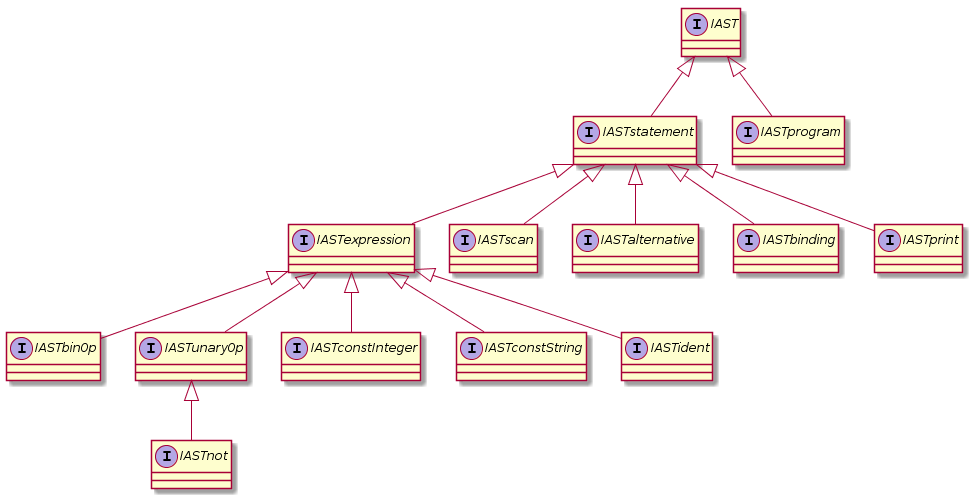
\includegraphics[scale=0.55]{./plantuml/ast_general_structure.png}
 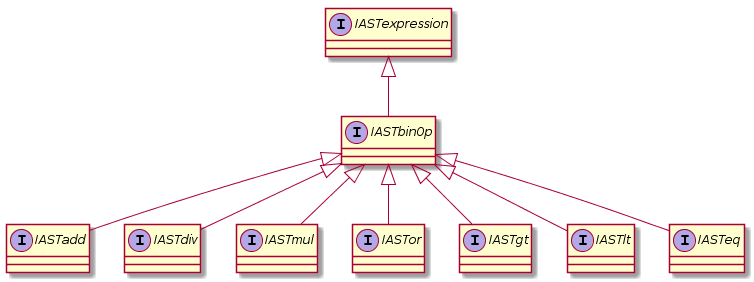
\includegraphics[scale=0.70]{./plantuml/ast_binop_structure.png}
 \begin{figure}
  \caption{Diagramme de classe de la structure générale}
 \end{figure}
\end{center}

La classe SUMListener réalise l'interface SUMgrammarListener, elle
permet d'appliquer une action à chaque trait reconnu du langage. La classe SUMParser
initialise le parser ANTLR et effectue la bonne séquence d'appels pour de construire l'arbre syntaxique abstrait.
Ces classes sont disponibles dans le dossier ./sum/SUM/src/sum/parser.

\section{Compilation vers le langage S-UM}
\subsection{Design Pattern Visitor}
Pour pouvoir parcourir et traiter chaque noeud de l'arbre syntaxique abstrait, nous avons utilisé le design pattern Visitor car il est
le mieux adapté lorsqu'on veut faire de l'interprétation/compilation en langage objet. Ainsi, tous les noeuds de l'AST possèdent
une méthode \textit{public void accept(IASTvisitor visitor)}. L'implantation de la classe Compiler permet d'effectuer la compilation de l'AST vers le langage.

\subsection{Description générale de la compilation (Classe Compiler)}
Voici une liste de variables et la description de leur utilité :
\begin{itemize}
 \item NO\_CONTEXT $\rightarrow$ Indique si l'évaluation retournée lors d'un appel à visit doit être stockée ou non.
 \item numInst $\rightarrow$ Représente le nombre d'instructions écrites (ce qui est utile pour l'alternative)
 \item env $\rightarrow$ Est une Map permettant de garder en mémoire le nom de la variable et l'indice du tableau dans lequel elle doit être
 stockée
 \item fos $\rightarrow$ est le flux de sortie
\end{itemize}

\subsection{Stockage des calculs}
On remarque qu'il n'y a que 8 registres disponibles, alors le stockage des calculs intermédiaires est limité : nous
devions trouver un moyen de stockage. Une propriété intéressante est que, lors du chargement du programme, seul le tableau[0] est occupé, ainsi on sait que l'indice des tableaux libres commence à 1. Alors, à l'aide d'une variable entière indVar, on connaît l'indice du tableau où se fera de la prochaine allocation de tableau, et à la fin de chaque allocation on incrémente indVar de 1. Il est important de noter que la désallocation ne se fera qu'à la sortie du programme : il n'y a aucune désalloctation en sortie de bloc. \\
Pour désallouer en sortie de bloc, il faudrait garder les indices des tableaux désalloués dans
une liste pour une réutilisation ultérieure lors de l'allocation. Hélàs, nous n'avons pas eu le temps de mettre en place cette implantation.
Chaque méthode visit possède un argument \textit{int context}. Si ce dernier est différent de \textit{NO\_CONTEXT}, il est l'indice du tableau 
dans lequel le résultat doit être stocké.
La méthode allocateVar() traduit en langage UM l'instruction d'allocation de taille 1, puisqu'on stocke uniquement une valeur.

\subsection{Traduction en instruction UM}
Traduire directement en binaire UM n'est pas chose aisée, c'est pour cela que nous avons défini des méthodes pour faciliter la traduction.
En voici un descriptif :
\begin{itemize}
 \item public void writeOperation(int op, int regA, int regB, int regC) $\rightarrow$ Permet d'écrire l'opération op avec les registres
 a, b et c en binaire UM dans le fichier de sortie, on écrit des bytes en utilisant des décalages. (Plus de détails dans le fichier Compiler
 en commentaire).
 \item public void writeSpecialOperation(int regA, int value) $\rightarrow$ Permet de charger une valeur non signée sur 25 bits dans 
 le registre A. (Plus de détails dans le fichier Compiler en commentaire)
 \item public void fetchIntoReg(int i, int reg) $\rightarrow$ Récupère une valeur simple située dans le plateau[i][0] (il s'agit de la valeur d'une variable) 
 et l'ajoute dans le registre reg.
 \item public void putIntoArray(int i, int reg) $\rightarrow$ Ajoute dans le plateau[i][0] la valeur dans le registre d'indice reg.
 \item public void allocateVar() $\rightarrow$ Alloue un plateau de taille 1 pour une variable.
\end{itemize}

\subsection{Egalité}
Ecrire les relations binaires a représenté une difficulté certaine. En effet, nous sommes très limités dans les opérations possibles.
Cependant, nous y sommes parvenus. Tout d'abord, remarquons la chose suivante : soit a un entier a. NAND(a,a) a pour effet d'inverser les bits. Les 0 deviennent des 1 et les 1 deviennent des
0. \\
Ainsi, nous observons que a + NAND(a,a) = 0b11..11, tous les bits sont positionnés à 1. \\
Donc en additionnant ce résultat à 1, on dépasse 32 bits et donc on retourne a 0b00..00. \\
Donc a + NAND(a,a) + 1 = 0b00..00. \\
On peut donc vérifier l'égalité a = b par : \\
si a + NAND(b,b) + 1 = 0b00..00 alors a = b sinon a != b.
\\ \\
Schéma de compilation : context = (expr1 = expr2);

\begin{verbatim}
  int contextarg1 = indVar++
  allocateVar()
  int contextarg2 = indVar++
  allocateVar()
  tableau[contextarg1][0] <- expr1
  tableau[contextarg2][0] <- expr2
  reg[0] <- tableau[contextarg1][0]
  reg[1] <- tableau[contextarg2][0]
  reg[2] <- NAND(1,1)
  reg[3] <- 1
  reg[2] <- reg[2] + reg[3]
  reg[0] <- reg[0] + reg[2]
  reg[1] <- 1
  reg[2] <- 0
  reg[1] <- if reg[0] = 0 then reg[1] else reg[2]
  tableau[context][0] <- reg[1]
\end{verbatim}

\subsection{Relation d'ordre: > et <}
Pour calculer la relation d'ordre a > b, il suffit de faire une division entière.
Si a/b > 0 alors la relation est vraie, mais il y a certaines mesures à prendre.
Il faut aussi vérifier le cas où a = b, nous réutilisons la code IASTeq. De plus, dans le cas où le dénominateur b = 0, on divise
par 0. Pour éviter cela, le calcul à considérer sera (a+1)/(b+1). Cela ne change pas la relation car si a/b > 0 alors (a+1)/(b+1) l'est aussi.
\\ \\
Schéma de compilation : context = (expr1 / expr2)
\begin{verbatim}
  int contextarg1 = indVar++
  allocateVar()
  int contextarg2 = indVar++
  allocateVar()
  
  tableau[contextarg1][0] <- expr1
  tableau[contextarg2][0] <- expr2
  reg[1] <- tableau[contextarg1][0]
  reg[2] <- tableau[contextarg2][0]
    
  //on ajoute 1 pour eviter la division par 0
  reg[3] <- 1
  reg[1] <- reg[1] + reg[3]
  reg[2] <- reg[2] + reg[3]
    
  //si reg[1]/reg[2] = 0 alors reg[1] < reg[2] car c'est une division entiere
  reg[3] <- reg[1]/reg[2]
  reg[0] <- 0
  reg[4] <- 1
  reg[0] <- if reg[3] != 0 then reg[4] else reg[0]
    
  //on verifie que reg[1] != reg[2]
  //ce sont les mêmes opérations que pour IASTeq
  reg[3] <- NAND(reg[2], reg[2])
  reg[4] <- 1
  reg[3] <- reg[3] + reg[4]
  reg[1] <- reg[3] + reg[1]
  reg[2] <- 1
  reg[3] <- 0
  
  reg[2] <- if reg[1] != 0 then reg[3] else reg[2]
  reg[1] <- 0
  reg[0] <- if reg[2] != 0 then reg[1] else reg[0]
    
  tableau[context][0] <- reg[0]
		
\end{verbatim}
Le code pour l'operation < est identique sauf qu'on change:
\begin{verbatim}
 tableau[contextarg2][0] <- expr1
 tableau[contextarg1][0] <- expr2
\end{verbatim}

\subsection{Or}
La traduction du OR se fait en calculant les membres gauche et droit.
A l'aide de l'opération 0 (mouvement conditionnel), nous déterminons si le résultat est 1 (vrai) ou faux (0).
\\ \\
Schéma de compilation : context = (expr1 OR expr2)
\begin{verbatim}
  int contextarg1 = indVar++
  allocateVar()
  int contextarg2 = indVar++
  allocateVar()
  tableau[contextarg1][0] <- expr1
  tableau[contextarg2][0] <- expr2
  reg[1] <- tableau[contextarg1][0]
  reg[2] <- tableau[contextarg2][0]
  reg[0] <- 0
  reg[3] <- 1
  //reg[1] et reg[2] contiennent le resultat de membre gauche et droit de OR
  //reg[0] contient 0, si reg[1] ou reg[2] contiennent la valeur != 0 alors
  //on met dans reg[0] la valeur 1, donc ceci est bien un OR
  reg[0] <- if reg[1] != 0 then reg[3] else reg[0]
  reg[0] <- if reg[1] != 0 then reg[2] else reg[0]
  tableau[context][0] <- reg[0]
\end{verbatim}

\subsection{And}
La traduction du And est très similaire à la traduction du Or. En effet, il y a uniquement une modification au niveau des mouvements
conditionnels.Nous faisons un ``chainage'' de mouvements conditionnels, ainsi reg[1] et reg[2] (registres qui contiennent le
résultat de l'évaluation des expressions) doivent tous les deux être différents de 0 pour que le résultat soit 1 (vrai).
\\ \\
Schéma de compilation : context = (expr1 AND expr2)
\begin{verbatim}
  int contextarg1 = indVar++
  allocateVar()
  int contextarg2 = indVar++
  allocateVar()
  tableau[contextarg1][0] <- expr1
  tableau[contextarg2][0] <- expr2
  reg[2] <- expr1
  reg[3] <- expr2
  reg[4] <- 1
  reg[5] <- 0
  reg[1] <- 0
  reg[0] <- 0
  //reg[2] et reg[3] contiennent le resultat du membre gauche et droit de AND
  //reg[1] = 0 si reg[2] != 0 alors reg[1] = 1
  //reg[0] = 0 si reg[3] != 0 alors reg[0] = reg[1]
  //donc si on a 0 AND 1, reg[0] = 0 etc
  reg[1] <- if reg[2] != 0 then reg[4] else reg[1]
  reg[0] <- if reg[3] != 0 then reg[1] else reg[0]
  tableau[context][0] <- reg[0]
\end{verbatim}

\subsection{Not}
La traduction du Not en UM est simple, on effectue un mouvement conditionnel : si la valeur est différent de 0 alors 1, 0 sinon.
\\ \\
Schéma de compilation : context = Not (expr)
\begin{verbatim}
  int argcontext = indVar++
  allocateVar()
  tableau[argcontext][0] <- expr
  reg[2] <- tableau[argcontext][0]
  reg[0] <- 1
  reg[1] <- 0
  //si le resultat est != 0 alors on met 1 sinon 0
  reg[0] <- if reg[2] != 0 then reg[1] else reg[0]
  tableau[context][0] <- reg[0]
\end{verbatim}

\subsection{Operation arithmétique}
Les opérations arithmétiques correspondent au chargement de valeur, l'application de l'opérande et au stockage du résultat.
\\ \\
Schéma de compilation : context = (expr1 [+*/] expr2)
\begin{verbatim}
  int contextarg1 = indVar++;
  allocateVar();
  int contextarg2 = indVar++;
  allocateVar();
  tableau[contextarg1][0] <- expr1
  tableau[contextarg2][0] <- expr2
  reg[0] <- tableau[contextarg1][0]
  reg[1] <- tableau[contextarg2][0]
  reg[2] <- reg[0] [+*/] reg[1]
  tableau[context][0] <- reg[2]
\end{verbatim}


\subsection{Alternative}
L'alternative a une compilation très intéressante à étudier. Tout d'abord, nous avons essayé de calculer dynamiquement le nombre
d'instructions à sauter pour les conditions, mais cela n'a pas été concluant. Ainsi avons-nous donc décidé d'allouer les blocs du 
conséquent et de l'alternative à une taille fixe, ce qui rend la détermination des sauts d'adresses plus simple.
En somme, l'alternative utilise les opérations de mouvements conditionnels pour déterminer quel saut il faut effectuer, mais aussi les
opérations de chargement de programme, qui permettent de produire des sauts d'instruction.
Nous utilisons ici une variable numInst afin de déterminer les adresses de sauts, numInst est incrémentée à chaque opération écrite.
\\ \\
Schéma de compilation : if expr1 then expr2 else expr3
\begin{verbatim}
  int DEFAULT_SIZE = 4096
  int condctx = indVar++
  allocateVar()
  tableau[condctx][0] <- expr1
  
  //suivant la valeur de la condition, on saute soit a l'adresse du then
  //ou alors a l'adresse du else
  //les blocs de then et else sont fixés, ce qui permet de calculer
  //directement les adresses de sauts
  reg[1] <- numInst+8 //then
  reg[0] <- numInst+8+DEFAULT_SIZE-1 //else
  reg[2] <- tableau[condctx][0]
  
  reg[0] <- if reg[2] != 0 then reg[1] else reg[0]
  reg[1] <- 0
  
  //on charge le programme tableau[reg[1]] et pointe sur la valeur de reg[0]
  //l'instruction qui sera éxécuté au tour prochain sera tableau[reg[1]][reg[0]]
  LOAD_PROG(reg[0], reg[1])
    
  //instructions du then
  int start = numInst;
  NO_CONTEXT <- expr2
    
  //saut hors du if
  reg[1] <- 0
  reg[0] <- start+2*DEFAULT_SIZE
  LOAD_PROG(reg[0],reg[1])
    
  //on remplit le reste du bloc avec des NOP
  while(numInst < start+DEFAULT_SIZE) {
    reg[0] <- 0
  }
    
  //instructions du else
  NO_CONTEXT <- expr3
    
  //on remplit le reste du bloc avec des NOP
  while(numInst < start+2*DEFAULT_SIZE) {
    reg[0] <- 0
  }
\end{verbatim}


\subsection{Binding}
Le binding est la combinaison d'une déclaration et d'une affectation de variable. Ainsi nous ajoutons la variable dans l'environnement de compilation, c'est-à-dire dans une map, le nom et l'indice
du tableau dans lequel on l'a attribuée. Si la variable est déclaré avec une expression le calcul de l'expression y sera stocké.
\\ \\
Schéma de compilation : let var = expr
\begin{verbatim}
  int varcontext = indVar++
  allocateVar()
  env.put(var, varcontext)
  if existExpr() then tableau[varcontext][0] <- expr
\end{verbatim}

\subsection{Ident}
Comme les identificateurs correspondent aux noms de variable, nous gardons dans l'environnement de compilation une map, contenant le nom de la variable
et l'indice du tableau, dans laquelle est stockée la variable.
\\ \\
Schéma de compilation : context = expr
\begin{verbatim}
  int varcontext = env.get(expr)
  reg[0] <- tableau[varcontext][0]
  tableau[context] <- reg[0]
\end{verbatim}


\subsection{Integer}
La traduction de la constante correspond au chargement de la valeur immédiate dans une case du tableau.
\\ \\
Schéma de compilation : context = expr
\begin{verbatim}
  reg[0] <- expr
  tableau[context][0] <- reg[0]
\end{verbatim}

\section{Tests}
Le jeux de tests se trouve dans le dossier ./tests, ce sont des tests unitaires de chaque trait du langage.
Nous effectuons principalement des tests avec des affichages attendus. Etant donné que l'affiche d'une expression est sous forme ASCII,
nous verifions dans la plupart des cas que la lettre retournée par l'appel correspond bien à la lettre attendue.
D'autres tests plus élaborés sont disponibles mais ne sont pas au format demandé. Ces tests se trouvent dans les sources 
du compilateur S-UM, dans le chemin ./sum/SUM/test.

\end{document}

